\documentclass[10pt,a4paper]{article}
\usepackage[margin=0.7in]{geometry}
\usepackage{multicol}
\usepackage{amsmath}
\usepackage{tikz}
\usepackage{enumitem}
\usepackage{titlesec}
\usepackage{booktabs}
\usepackage{fontspec}

% Compact formatting
\setlength{\columnsep}{0.7cm}
\setlength{\parindent}{0pt}
\setlength{\parskip}{0.12cm}
\titlespacing{\section}{0pt}{0.4cm}{0.15cm}
\titlespacing{\subsection}{0pt}{0.25cm}{0.08cm}
\titlespacing{\subsubsection}{0pt}{0.2cm}{0.05cm}

% Custom section style
\titleformat{\section}{\large\bfseries}{}{0em}{}
\titleformat{\subsection}{\normalsize\bfseries}{}{0em}{}
\titleformat{\subsubsection}{\normalsize\bfseries\itshape}{}{0em}{}

\begin{document}

\begin{center}
{\LARGE \textbf{Firm Decisions, Revenue \& Market Structure}}\\[0.15cm]
{\normalsize \textit{Topic 7: Optimal Input Choice, Profit Maximization, and Market Power}}\\[0.15cm]
\hrule
\end{center}
\vspace{-0.3cm}

\begin{multicols}{2}
\footnotesize

% ============================================================================
% PART 1: DEFINITIONS AND CORE CONCEPTS
% ============================================================================
\section*{1. Core Definitions}

\subsection*{Isoquants and Isocosts}
\textbf{Isoquant:} An \textbf{isoquant} (Equal-Quantity curve) shows all combinations of two inputs (typically Labor $L$ and Capital $K$) that produce the \textbf{same level of output}. It is the firm's analog of the consumer's indifference curve.
\[
Q = f(L, K) = \bar{Q} \quad \text{(constant)}
\]

\textbf{Isocost Line:} An \textbf{isocost} (Equal-Cost line) shows all combinations of $L$ and $K$ that cost the firm the \textbf{same total expenditure}.
\[
C = wL + rK \quad \Rightarrow \quad K = \frac{C}{r} - \frac{w}{r}L
\]
Where: $w$ = wage rate, $r$ = rental rate of capital. Slope of isocost = $-w/r$ (relative input price ratio).

\subsection*{Least Cost Combination (Optimal Input Choice)}
The firm minimizes cost for a given output level by choosing $L$ and $K$ where the isoquant is \textbf{tangent} to the lowest possible isocost line:
\[
MRTS_{LK} = \frac{MP_L}{MP_K} = \frac{w}{r}
\]
\textbf{Marginal Rate of Technical Substitution (MRTS):} The rate at which the firm can substitute $L$ for $K$ while keeping output constant. It equals the ratio of marginal products. At optimum, the last dollar spent on each input yields the same additional output.

\subsection*{Revenue Concepts}
\begin{itemize}[leftmargin=*,nosep]
    \item \textbf{Total Revenue (TR):} $TR = P \times Q$.
    \item \textbf{Average Revenue (AR):} $AR = TR/Q = P$. The demand curve \textbf{is} the AR curve.
    \item \textbf{Marginal Revenue (MR):} $MR = \Delta TR / \Delta Q = d(TR)/dQ$. Additional revenue from selling one more unit.
\end{itemize}

\textbf{Relationship between AR and MR:}
\begin{itemize}[leftmargin=*,nosep]
    \item \textbf{Perfect Competition:} Firm is a price-taker. $P$ is constant. $AR = MR = P$ (horizontal demand curve).
    \item \textbf{Imperfect Competition (Monopoly, Monopolistic Competition, Oligopoly):} Firm faces downward-sloping demand. To sell more, price must fall on \textbf{all} units. $MR < AR = P$. $MR$ curve lies below the demand (AR) curve.
    \[
    MR = P \left(1 + \frac{1}{E_d}\right) \quad \text{or} \quad MR = P \left(1 - \frac{1}{|E_d|}\right)
    \]
    Since $E_d < 0$, $MR < P$ for downward-sloping demand.
\end{itemize}

% ============================================================================
% PART 2: HOW TO REMEMBER
% ============================================================================
\section*{2. Memory Triggers and Conceptual Anchors}

\begin{itemize}[leftmargin=*,nosep]
    \item \textbf{Isoquant = Same Quantity = Production IC:} Just like indifference curves, but for output. Higher isoquant = more output.
    \item \textbf{Isocost = Same Cost = Budget Line:} Just like the consumer's budget line, but for the firm. Slope $= -w/r$ (relative price of labor).
    \item \textbf{Least Cost Tangency:} $MRTS = w/r$. The rate at which you \textit{can} trade machines for workers in the market (price ratio) equals the rate at which you \textit{need} to trade them to keep output constant (MP ratio). ``The market trade-off matches the technical trade-off.''
    \item \textbf{MR vs AR in Imaginary Markets:}
    \begin{itemize}[nosep]
        \item \textbf{Perfect Competition:} ``I can sell all I want at the market price.'' $MR = P$. AR curve is a flat line.
        \item \textbf{Monopoly:} ``To sell more, I must lower the price on EVERY unit.'' $MR$ is below $P$, steeper than demand. ``Price cut bleeds revenue from inframarginal units.''
    \end{itemize}
    \item \textbf{Profit Max Rule:} $MR = MC$. If $MR > MC$: produce more (adds more to revenue than cost). If $MR < MC$: produce less. At $MR = MC$, profit is maximized. \textbf{This rule is universal across ALL market structures.}
    \item \textbf{Market Structure Spectrum -- ``Many to One'':}
    \begin{itemize}[nosep]
        \item \textbf{Perfect Competition:} Infinite firms, identical product.
        \item \textbf{Monopolistic Competition:} Many firms, differentiated product.
        \item \textbf{Oligopoly:} Few firms, strategic interaction.
        \item \textbf{Monopoly:} One firm, no close substitutes.
    \end{itemize}
    \item \textbf{Game Theory in Oligopoly:} ``Prisoner's Dilemma'' -- both firms could earn higher profits by cooperating (high prices), but each has an incentive to cheat (lower price), leading to a worse joint outcome.
\end{itemize}

% ============================================================================
% PART 3: MATHEMATICAL FRAMEWORK
% ============================================================================
\section*{3. Mathematical Formulation}

\subsection*{Cost Minimization Problem}
\[
\min_{L, K} \; wL + rK \quad \text{s.t.} \quad f(L, K) = Q_0
\]
Lagrangian: $\mathcal{L} = wL + rK + \lambda (Q_0 - f(L, K))$.
First-order conditions:
\[
w - \lambda \frac{\partial f}{\partial L} = 0; \quad r - \lambda \frac{\partial f}{\partial K} = 0; \quad Q_0 = f(L, K)
\]
Dividing: $\frac{w}{r} = \frac{MP_L}{MP_K} = MRTS_{LK}$.

The solution $L^*(w, r, Q_0)$, $K^*(w, r, Q_0)$ are \textbf{conditional factor demands}. The cost function $C(w, r, Q_0) = wL^* + rK^*$.

\subsection*{Revenue Functions and MR}
For linear demand $P = a - bQ$:
\[
TR = P \cdot Q = aQ - bQ^2
\]
\[
AR = \frac{TR}{Q} = a - bQ = P
\]
\[
MR = \frac{d(TR)}{dQ} = a - 2bQ
\]
Note: $MR$ has twice the slope of the demand curve ($-2b$ vs. $-b$). Both share same vertical intercept ($a$ on the price axis).

\textbf{MR in terms of elasticity:}
\[
MR = \frac{d(TR)}{dQ} = P + Q \cdot \frac{dP}{dQ} = P \left(1 + \frac{Q}{P} \cdot \frac{dP}{dQ}\right) = P\left(1 + \frac{1}{E_d}\right)
\]

\subsection*{Profit Maximization Condition}
\[
\pi(Q) = TR(Q) - TC(Q)
\]
First-order condition: $\frac{d\pi}{dQ} = MR - MC = 0 \Rightarrow \mathbf{MR = MC}$.
Second-order condition: $\frac{d^2\pi}{dQ^2} < 0 \Rightarrow \frac{d(MR)}{dQ} < \frac{d(MC)}{dQ}$ (slope of MR < slope of MC at optimum).

\textbf{Market-Specific MR:}
\begin{itemize}[nosep]
    \item \textbf{Perfect Competition:} $P$ constant, $MR = P$. Thus condition: $P = MC$.
    \item \textbf{Monopoly:} $MR = P(1 + 1/E_d) = MC$. Since $E_d < 0$, $P > MC$. Markup: $\frac{P - MC}{P} = \frac{1}{|E_d|}$ (Lerner Index).
\end{itemize}

\subsection*{Market Structures Summary Equations}
\begin{center}
\begin{tabular}{@{}p{2cm}p{1.8cm}p{2.2cm}@{}}
\toprule
\textbf{Structure} & \textbf{Demand} & \textbf{Profit Max} \\
\midrule
Perfect Comp. & $P = AR = MR$ (flat) & $P = MC$ ($Q$ where $P=MC$) \\
Monopoly & $P > MR$ (downward) & $MR = MC$, then $P > MC$ \\
Monop. Comp. & $P > MR$ (downward) & $MR = MC$ (SR profit, LR break-even) \\
Oligopoly & Downward (\& interdependent) & $MR = MC$ given rivals' strategies \\
\bottomrule
\end{tabular}
\end{center}

% ============================================================================
% PART 4: GRAPHICAL ANALYSIS
% ============================================================================
\section*{4. Graphical Illustrations}

\subsection*{Isocost-Isoquant: Least Cost Combination}
\begin{center}
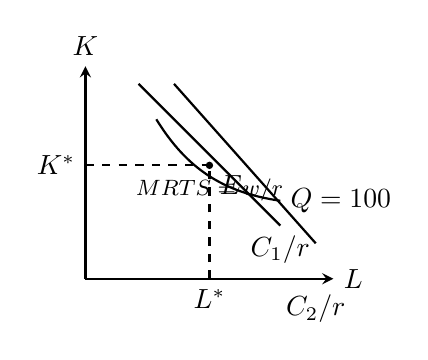
\begin{tikzpicture}[scale=0.45, thick, >=stealth]
    \draw[->] (0,0) -- (7,0) node[right] {$L$};
    \draw[->] (0,0) -- (0,6) node[above] {$K$};
    % Isocost lines
    \draw[thick] (1.5,5.5) -- (5.5,1.5) node[below] {$C_1 / r$};
    \draw[thick] (2.5,5.5) -- (6.5,1) node[below=15pt] {$C_2 / r$};
    % Isoquant
    \draw[thick] (2,4.5) to[bend right=25] (5.5,2.2) node[right] {$Q=100$};
    % Tangency point
    \filldraw (3.5,3.2) circle (2pt) node[below right] {$E$};
    \node at (3.5,2.5) {\footnotesize $MRTS = w/r$};
    \draw[dashed] (3.5,0) node[below] {$L^*$} -- (3.5,3.2);
    \draw[dashed] (0,3.2) node[left] {$K^*$} -- (3.5,3.2);
\end{tikzpicture}
\end{center}
\textit{Point $E$ minimizes cost for producing $Q=100$. The firm cannot afford the $C_2$ isocost; $C_1$ is affordable but produces less than 100. At E, $MRTS = w/r$.}

\subsection*{MR and AR for a Monopolist (Linear Demand)}
\begin{center}
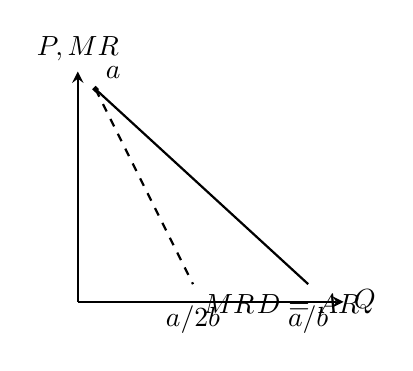
\begin{tikzpicture}[scale=0.45, thick, >=stealth]
    \draw[->] (0,0) -- (7.5,0) node[right] {$Q$};
    \draw[->] (0,0) -- (0,6.5) node[above] {$P, MR$};
    % Demand (AR) curve
    \draw[thick] (0.5,6) -- (6.5,0.5) node[below] {$D = AR$};
    % MR curve (twice the slope)
    \draw[thick, dashed] (0.5,6) -- (3.25,0.5) node[below right] {$MR$};
    \filldraw (0.5,6) circle (1.5pt) node[above right] {$a$};
    \node at (3.25,-0.5) {$a/2b$}; \node at (6.5,-0.5) {$a/b$};
\end{tikzpicture}
\end{center}
\textit{For $P = a - bQ$, $MR = a - 2bQ$. MR is twice as steep and crosses the x-axis at half the quantity.}

\subsection*{Profit Maximization: MR = MC}
\begin{center}
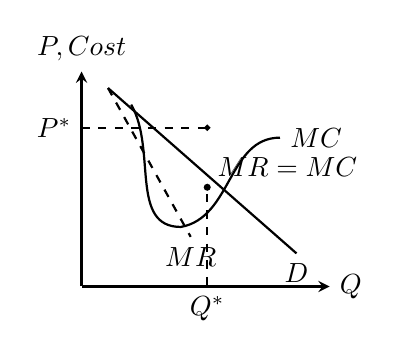
\begin{tikzpicture}[scale=0.42, thick, >=stealth]
    \draw[->] (0,0) -- (7.5,0) node[right] {$Q$};
    \draw[->] (0,0) -- (0,6.5) node[above] {$P, Cost$};
    \draw[thick] (0.8,6) -- (6.5,1) node[below] {$D$};
    \draw[thick, dashed] (0.8,6) -- (3.3,1.5) node[below] {$MR$};
    \draw[thick] (1.5,5.5) to[out=300, in=180] (3,1.8) to[out=10, in=180] (6,4.5) node[right] {$MC$};
    \filldraw (3.8,3) circle (2pt) node[above right] {$MR=MC$};
    \draw[dashed] (3.8,2.8) -- (3.8,0) node[below] {$Q^*$};
    \draw[dashed] (0,4.8) node[left] {$P^*$} -- (3.8,4.8);
    \filldraw (3.8,4.8) circle (1.5pt);
\end{tikzpicture}
\end{center}
\textit{Firm produces $Q^*$ where $MR=MC$. Price $P^*$ is read from the demand curve at $Q^*$. Shaded area (if ATC was drawn) = profit.}

% ============================================================================
% PART 5: MARKET STRUCTURES - DETAILED ANALYSIS
% ============================================================================
\section*{5. Market Structure Models (Detailed)}

\subsection*{Perfect Competition}
\textbf{Characteristics:}
\begin{itemize}[leftmargin=*,nosep]
    \item \textbf{Large number} of buyers and sellers -- no single agent affects price.
    \item \textbf{Homogeneous} product -- perfect substitutes.
    \item \textbf{Free entry and exit} -- zero barriers.
    \item \textbf{Perfect information} -- all agents know prices and technology.
    \item Firm is a \textbf{price taker}.
\end{itemize}

\textbf{Short-Run Equilibrium:} $P = MC$. Firm may earn \textbf{supernormal profit} ($P > ATC$), \textbf{normal profit} ($P = ATC$), or operate at \textbf{loss} ($P < ATC$ but $P > AVC$) to minimize loss. Shutdown if $P < AVC$.

\textbf{Long-Run Equilibrium:} Free entry/exit drives economic profit to zero. $P = MC = \min ATC$. \textbf{Allocative efficiency} ($P = MC$) and \textbf{productive efficiency} ($P = \min ATC$) achieved.

\subsection*{Monopoly}
\textbf{Characteristics:}
\begin{itemize}[leftmargin=*,nosep]
    \item \textbf{Single seller}, no close substitutes.
    \item \textbf{High barriers to entry} (legal, patents, control of resources, natural monopoly).
    \item Firm is a \textbf{price maker}, faces market demand.
\end{itemize}

\textbf{Equilibrium:} $MR = MC$, then charge $P^*$ from demand curve. $P^* > MC$. \textbf{Deadweight loss} exists (underproduction relative to competitive ideal).

\textbf{Price Discrimination:} Monopolist can increase profit by charging different prices to different consumers:
\begin{itemize}[nosep]
    \item 1st Degree (Perfect): Each consumer pays their maximum willingness to pay. No consumer surplus remains.
    \item 2nd Degree: Different prices for different quantities (bulk discounts, block pricing).
    \item 3rd Degree: Different prices in different market segments based on elasticity (e.g., student/senior discounts).
\end{itemize}

\subsection*{Monopolistic Competition (Chamberlin)}
\textbf{Characteristics:}
\begin{itemize}[leftmargin=*,nosep]
    \item \textbf{Many sellers}, free entry/exit.
    \item \textbf{Differentiated products} -- perceived or real quality differences, branding, location. Each firm has slight market power.
    \item Demand curve is \textbf{highly elastic} but downward-sloping.
\end{itemize}

\textbf{Short-Run:} Like a mini-monopoly. $MR = MC$, earns profit/loss.

\textbf{Long-Run:} Entry drives profit to zero ($P = ATC$). But unlike perfect competition, $P > MC$ (not allocatively efficient) and $P > \min ATC$ (excess capacity -- firm produces left of minimum efficient scale). Consumers pay higher price but enjoy \textbf{variety}.

\subsection*{Oligopoly and Game Theory}
\textbf{Characteristics:}
\begin{itemize}[leftmargin=*,nosep]
    \item \textbf{Few dominant firms}; high barriers to entry.
    \item Products may be homogeneous (steel, oil) or differentiated (automobiles, smartphones).
    \item \textbf{Strategic interdependence} -- each firm's decisions depend on rivals' expected actions. Modeled using \textbf{Game Theory}.
\end{itemize}

\textbf{Cournot Model (Quantity Competition):} Firms choose output simultaneously. Each firm's optimal output depends on rival's output. Equilibrium: each correctly guesses the other's output; no incentive to deviate. Market price between competitive and monopoly levels.

\textbf{Bertrand Model (Price Competition):} Firms set prices simultaneously. With homogeneous goods, undercutting drives price down to $MC$ (paradoxically, two firms can yield competitive outcome).

\textbf{Game Theory -- Prisoner's Dilemma (Oligopoly Pricing):}
Two firms (A and B) decide: \textbf{High Price (Cooperate)} or \textbf{Low Price (Defect)}.
\begin{center}
\begin{tabular}{cc|c|c|}
\multicolumn{2}{c}{} & \multicolumn{2}{c}{\textbf{Firm B}} \\
\multicolumn{2}{c}{} & High Price & Low Price \\
\cline{3-4}
\multirow{2}{*}{\textbf{Firm A}} & High Price & (10, 10) & (2, 15) \\
\cline{3-4}
& Low Price & (15, 2) & (5, 5) \\
\cline{3-4}
\end{tabular}
\end{center}
\textit{(Payoffs in millions. A's payoff first, B's second.)}
\begin{itemize}[nosep]
    \item \textbf{Dominant Strategy for Each:} Low Price (Defect). Regardless of rival's choice, defecting yields higher payoff.
    \item \textbf{Nash Equilibrium:} (Low, Low) $\to$ (5, 5).
    \item \textbf{Cooperative Outcome:} (High, High) $\to$ (10, 10) is better for both but unstable because each has incentive to cheat.
    \item This explains why cartels (like OPEC) tend to break down without enforcement.
\end{itemize}

\textbf{Collusion and Cartels:} Firms may collude (jointly set $MR = MC$, act like a monopoly) to maximize joint profits. Illegal in most jurisdictions (antitrust laws). Cartels face incentive to cheat (prisoner's dilemma) and must have enforcement mechanisms.

\textbf{Kinked Demand Curve (Sweezy Model):} Explains price rigidity in oligopoly. Competitors match price cuts but not price increases. Creates a kink in the demand curve and a discontinuous MR curve; MC can shift within the gap without changing optimal price.

% ============================================================================
% PART 6: EXTENSIVE CASE STUDIES
% ============================================================================
\section*{6. Comprehensive Case Studies}

\subsection*{Case Study 1: OPEC and the Prisoner's Dilemma of Oil Cartels (1973--2024)}

\textbf{Background:} The Organization of the Petroleum Exporting Countries (OPEC), formed in 1960, is the world's most famous (and only partially successful) cartel. It controls roughly 40\% of global oil production. OPEC's core dilemma is the classic \textbf{prisoner's dilemma}: all members collectively benefit from restricting output to keep prices high, but each member individually benefits from cheating and producing more than its quota.

\textbf{Cooperative Equilibrium (Cartel Profit Maximization):}
OPEC acts as a \textbf{multi-plant monopolist}. It sets total output where $MR_{\text{world oil}} = MC_{\text{aggregate}}$ and allocates quotas to members. The collective monopoly price ($P_m$) is high; each member earns supernormal profits.

\textbf{Incentive to Cheat:}
Each member country faces an individual $P > MC$ (since P is set at monopoly level). If a single country (e.g., Saudi Arabia in some periods, Iraq, Venezuela) secretly increases production above its quota, it sells more barrels at the high monopoly price, increasing its own revenue. The price effect (small price drop from extra output) is borne by \textit{all} members, while the quantity effect (extra revenue) accrues to the cheater alone. This is the \textbf{free-rider problem} in cartels.

\textbf{Historical Evidence: Prisoner's Dilemma in Action.}

\textit{Episode 1: 1973 Oil Embargo \& 1970s Success.} OPEC successfully cut production, quadrupling prices. Members initially cooperated. The high price held because demand was highly inelastic in the short run.

\textit{Episode 2: 1980s Collapse.} As high prices persisted, demand became more elastic (conservation, fuel-efficient cars). Non-OPEC supply expanded (North Sea, Alaska). OPEC members, facing reduced market share, began \textbf{cheating on quotas}. Saudi Arabia, traditionally the ``swing producer,'' cut its output to defend prices alone, but other members overproduced. By 1986, oil prices crashed from \$30 to below \$10/barrel. The cartel had collapsed into the non-cooperative Nash equilibrium (high output, low price).

\textit{Episode 3: 2020 Price War (Saudi Arabia vs. Russia).} After COVID-19 crushed demand, OPEC+ (OPEC plus Russia) attempted to coordinate production cuts. Russia refused to cut its quota. Saudi Arabia responded by flooding the market (a strategic play in the repeated game), driving prices negative briefly (WTI futures hit -\$37). This was a \textbf{punishment strategy} in a repeated game: Saudi Arabia signaled its willingness to endure short-term pain to enforce long-term cooperation. The cartel subsequently agreed to historic production cuts.

\textit{Episode 4: 2022--2024 Coordination Amid Geopolitical Tension.} The Russia-Ukraine war disrupted supply. OPEC+ maintained cuts, demonstrating that when external shocks align members' interests (everyone gains from high prices with limited ability to expand output), cooperation can hold. However, internal tensions (smaller African producers wanting to produce more, UAE seeking higher baseline quotas) persist.

\textbf{Game Theory Lessons:}
\begin{enumerate}[leftmargin=*,nosep]
    \item \textbf{Static game (one-shot):} Defection (cheating) is the dominant strategy $\to$ cartel unstable.
    \item \textbf{Repeated game:} If the game is infinitely repeated, \textbf{tit-for-tat} strategies (cooperate if rival cooperated last period; defect if they defected) can sustain cooperation if the discount rate is low enough (future profits matter). Saudi Arabia has often played this role.
    \item \textbf{Monitoring and Punishment:} Effective cartels need transparency (observing output) and enforcement mechanisms. OPEC's monitoring has been historically weak, leading to endemic cheating.
    \item \textbf{Market Structure evolves:} Entry of new producers (shale oil, renewables) erodes cartel power. The shale revolution made non-OPEC supply more elastic, limiting OPEC's ability to raise prices without losing significant market share.
\end{enumerate}

\textbf{Economic Concepts Demonstrated:} Prisoner's dilemma, dominant strategy, Nash equilibrium, cartel instability, repeated game strategies, elasticity and monopoly power.

\subsection*{Case Study 2: The Streaming Wars -- Oligopoly and Strategic Interaction (Netflix, Disney+, Amazon Prime, 2019--2024)}

\textbf{Background:} The global streaming video market evolved from a near-monopoly (Netflix, 2015--2019) to an \textbf{oligopoly} with the entry of deep-pocketed competitors: Disney+ (2019), Apple TV+ (2019), HBO Max (2020, now Max), Amazon Prime Video, and others. The industry exemplifies non-price competition, strategic investment, and game-theoretic behavior.

\textbf{Market Structure Analysis:}
\begin{itemize}[leftmargin=*,nosep]
    \item \textbf{Few major firms (Oligopoly):} Netflix, Disney+, Amazon Prime, Max, Apple TV+ dominate. High concentration but no single monopoly.
    \item \textbf{High barriers to entry:} Massive content spending (billions annually for original programming), technology infrastructure, and subscriber base lock-in. New entrants need enormous capital.
    \item \textbf{Differentiated products:} Each platform differentiates by exclusive content (Netflix: \textit{Stranger Things}; Disney+: Marvel, Star Wars; Amazon: \textit{LOTR: Rings of Power}; Apple: \textit{Ted Lasso}).
    \item \textbf{Strategic interdependence:} Pricing, content spending, and bundling decisions are made with rivals' expected reactions in mind.
\end{itemize}

\textbf{Game Theory: A Content Spending ``Arms Race''}

The competition resembles a \textbf{prisoner's dilemma} in content investment.

\textit{Scenario:} Two firms (Netflix and Disney+) must choose: \textbf{High Content Budget (\$15B+)} or \textbf{Moderate Content Budget (\$8B)}.

\begin{center}
\begin{tabular}{cc|c|c|}
\multicolumn{2}{c}{} & \multicolumn{2}{c}{\textbf{Disney+}} \\
\multicolumn{2}{c}{} & High Budget & Moderate Budget \\
\cline{3-4}
\multirow{2}{*}{\textbf{Netflix}} & High Budget & (5, 4) & (9, 2) \\
\cline{3-4}
& Moderate Budget & (2, 9) & (7, 7) \\
\cline{3-4}
\end{tabular}
\end{center}
\textit{(Hypothetical profit indices. High spending $\to$ high subscriber appeal but high costs.)}

\begin{itemize}[leftmargin=*,nosep]
    \item If both choose \textbf{Moderate Budget}, they earn reasonable profits (7, 7). Total industry profitability is high.
    \item However, if one spends \textbf{High} while the other spends Moderate, the high-spender captures market share and subscriber growth (9 vs. 2 for the rival).
    \item \textbf{Dominant Strategy?} If each fears the rival will spend high, the best response is also to spend high (to avoid being left behind). The Nash Equilibrium is (High, High) with profits (5, 4) -- lower for both than (Moderate, Moderate).
    \item This is precisely what happened: Netflix, Disney, Amazon, and Apple all ramped up content spending to \$10--\$20 billion per year, eroding profitability. Netflix's free cash flow was negative for years due to this arms race.
\end{itemize}

\textbf{Strategic Behavior Observed:}
\begin{enumerate}[leftmargin=*,nosep]
    \item \textbf{Non-Price Competition:} Price competition is muted (prices crept up slowly). Primary competition is through \textbf{content quality/exclusivity} (differentiation) and \textbf{marketing}. This is classic monopolistic competition / oligopoly behavior -- avoid price wars, compete on non-price dimensions.
    \item \textbf{Entry Deterrence / Pre-emption:} Netflix's massive early spending on originals was partly a \textbf{first-mover strategy} to build a content library so large that rivals would find it difficult to compete (barrier to entry).
    \item \textbf{Bundling (Economies of Scope):} Disney+ bundled with Hulu and ESPN+; Amazon Prime Video bundled with Prime shipping; Apple TV+ bundled with Apple One. Bundling leverages market power across multiple markets to lock in subscribers (reduce churn).
    \item \textbf{Reaction Functions in Pricing:} When Netflix raised prices (2022--2023), Disney+ followed shortly after. This is consistent with \textbf{price leadership} or \textbf{conscious parallelism} -- a form of tacit collusion where firms monitor and match price moves without explicit agreement.
    \item \textbf{Churn and Password Sharing (2023):} Netflix's crackdown on password sharing was a \textbf{strategic move} to increase revenue from existing content without additional spending (raising MR without raising MC). Competitors watched; if successful, they'll adopt similar strategies (a ``best-response'' imitation).
    \item \textbf{Ad-Supported Tiers (2023--2024):} Both Netflix and Disney+ introduced cheaper ad-supported plans. This is \textbf{third-degree price discrimination}: segmenting consumers by willingness to pay (price-sensitive consumers accept ads; less price-sensitive pay for ad-free). This increases total revenue without losing high-value subscribers. In game terms, it's a new strategic variable introduced simultaneously.
\end{enumerate}

\textbf{Evolution Toward a New Equilibrium:}
By 2023--2024, the industry showed signs of moving from the ``content arms race'' to a more \textbf{cooperative equilibrium} (at least tacitly):
\begin{itemize}[leftmargin=*,nosep]
    \item Content spending growth slowed; firms emphasized ``profitability over growth.''
    \item Price increases became coordinated signals.
    \item Some content licensing resumed: Netflix began licensing HBO shows; a move toward cooperation (expanding pie) rather than pure competition.
    \item This suggests the industry may be evolving from a non-cooperative prisoner's dilemma outcome toward a \textbf{tacitly collusive} outcome, potentially increasing joint profits.
\end{itemize}

\textbf{Economic Lessons:}
\begin{enumerate}[leftmargin=*,nosep]
    \item \textbf{Oligopoly theory} accurately predicts arms races in non-price competition (advertising, R\&D, content) and the tragedy of excessive spending.
    \item \textbf{Differentiation} is the central strategy: firms create market power (downward-sloping demand) through unique content, even in a crowded market.
    \item \textbf{Repeated interaction} and signaling can lead toward tacit collusion, reducing competition over time.
    \item \textbf{Game theory frameworks} (prisoner's dilemma, reaction functions, strategic complements/substitutes) are essential for understanding and predicting firm behavior in concentrated markets.
\end{enumerate}

\columnbreak

% ============================================================================
% PART 7: EXAM QUESTIONS
% ============================================================================
\section*{7. Exam Questions \& Model Answers}

\subsection*{Question 1: Cost Minimization (Isocost-Isoquant)}
\textbf{A firm's production function is $Q = L^{0.5} K^{0.5}$. Wage $w = 10$, rental $r = 40$. The firm wants to produce $Q = 100$ units.}
\textbf{(a) Find the optimal ($L^*, K^*$) combination that minimizes cost.}
\textbf{(b) Calculate the minimum total cost.}
\textbf{(c) Show that at the optimum, $MRTS = w/r$.}

\vspace{0.05cm}
\textbf{Solution:}
\vspace{0.05cm}
\textbf{(a)} $MP_L = 0.5 L^{-0.5} K^{0.5}$, $MP_K = 0.5 L^{0.5} K^{-0.5}$.
$MRTS = MP_L/MP_K = K/L$. Set $K/L = w/r = 10/40 = 1/4 \Rightarrow K = 0.25L$.
Output: $Q = L^{0.5} (0.25L)^{0.5} = L^{0.5} \cdot 0.5 L^{0.5} = 0.5L = 100 \Rightarrow \mathbf{L=200}$. Then $\mathbf{K = 0.25(200) = 50}$.

\textbf{(b)} $TC = 10(200) + 40(50) = 2000 + 2000 = \mathbf{4000}$.

\textbf{(c)} At optimum: $K/L = 50/200 = 0.25 = 1/4 = 10/40 = w/r$. Verified. $\checkmark$

\vspace{0.2cm}

\subsection*{Question 2: Profit Maximization (Monopoly)}
\textbf{Monopolist faces: Demand $P = 120 - 2Q$, Total Cost $TC = 100 + 4Q + Q^2$.}
\textbf{(a) Find profit-maximizing $Q$, $P$, and $\pi$.}
\textbf{(b) Compare with perfectly competitive outcome ($P = MC$).}
\textbf{(c) Calculate consumer surplus, producer surplus, and deadweight loss under monopoly.}

\vspace{0.05cm}
\textbf{Solution:}
\vspace{0.05cm}
\textbf{(a)} $TR = (120 - 2Q)Q = 120Q - 2Q^2$. $MR = 120 - 4Q$.
$MC = 4 + 2Q$. Set $MR = MC$: $120 - 4Q = 4 + 2Q \Rightarrow 116 = 6Q \Rightarrow \mathbf{Q^* = 19.33}$.
$P^* = 120 - 2(19.33) = \mathbf{81.33}$.
$TR = 120(19.33) - 2(19.33)^2 \approx 1573.3$. $TC = 100 + 4(19.33) + (19.33)^2 \approx 550.9$.
$\pi = 1573.3 - 550.9 = \mathbf{1022.4}$.

\textbf{(b)} Competitive: $P = MC$. $120 - 2Q = 4 + 2Q \Rightarrow 116 = 4Q \Rightarrow Q_c = 29$.
$P_c = 120 - 2(29) = 62$. Monopolist produces less (19.33 vs. 29) at higher price (81.33 vs. 62).

\textbf{(c)} Under monopoly:
\begin{itemize}[nosep]
    \item CS = area below demand, above $P^*$, up to $Q^*$. $CS = \frac{1}{2}(120 - 81.33)(19.33) = \frac{1}{2}(38.67)(19.33) \approx 373.8$.
    \item PS (monopoly) = $TR - TVC = 1573.3 - (4(19.33) + 19.33^2) = 1573.3 - 450.9 = 1122.4$. (Note: TFC excluded from PS; or PS = $\pi + TFC = 1022.4 + 100 = 1122.4$.)
    \item Competitive CS = $\frac{1}{2}(120-62)(29) = \frac{1}{2}(58)(29) = 841$.
    \item Competitive PS = $\frac{1}{2}(62-4)(29) = 841$ (since MC at Q=0 is 4).
    \item DWL = Competitive Total Surplus $-$ Monopoly Total Surplus = $(841+841) - (373.8+1122.4) = 1682 - 1496.2 = \mathbf{185.8}$.
\end{itemize}

\vspace{0.2cm}

\subsection*{Question 3: Game Theory (Oligopoly)}
\textbf{Two firms play a simultaneous pricing game. Each chooses High Price or Low Price. Payoff matrix (A's profit, B's profit in \$M):}

\begin{center}
\begin{tabular}{cc|c|c|}
\multicolumn{2}{c}{} & \multicolumn{2}{c}{Firm B} \\
\multicolumn{2}{c}{} & High & Low \\
\cline{3-4}
\multirow{2}{*}{Firm A} & High & (8, 8) & (1, 12) \\
\cline{3-4}
& Low & (12, 1) & (3, 3) \\
\cline{3-4}
\end{tabular}
\end{center}

\textbf{(a) Find the Nash equilibrium (or equilibria).}
\textbf{(b) Is this a prisoner's dilemma? Explain.}
\textbf{(c) If the game is repeated infinitely with a discount factor $\delta = 0.9$, can cooperation (High, High) be sustained using a Grim Trigger strategy? Show calculation.}

\vspace{0.05cm}
\textbf{Solution:}
\vspace{0.05cm}
\textbf{(a)}
If A chooses High, B compares 8 (High) vs 12 (Low) $\to$ B chooses Low.
If A chooses Low, B compares 1 (High) vs 3 (Low) $\to$ B chooses Low.
\textit{Low is dominant strategy for B.} By symmetry, Low is also dominant for A.
\textbf{Nash Equilibrium: (Low, Low) with payoffs (3, 3).}

\textbf{(b)} Yes, it is a prisoner's dilemma. The cooperative outcome (High, High) yields (8, 8), which is \textbf{Pareto superior} to the Nash equilibrium (3, 3). But each player has a dominant strategy to defect, resulting in a worse outcome for both.

\textbf{(c)} Grim Trigger: Cooperate (High) in period 1. If rival ever defects, switch to (Low) forever.
Cooperating yields: $8 + 8\delta + 8\delta^2 + \dots = \frac{8}{1-\delta}$.
Defecting today yields: $12 + 3\delta + 3\delta^2 + \dots = 12 + \frac{3\delta}{1-\delta}$.
Cooperation sustainable if: $\frac{8}{1-\delta} \geq 12 + \frac{3\delta}{1-\delta}$.
With $\delta = 0.9$: LHS = $8/(0.1) = 80$. RHS = $12 + 3(0.9)/(0.1) = 12 + 27 = 39$.
Since $80 > 39$, cooperation \textbf{can be sustained}. The threat of future punishment is credible and severe enough ($\delta$ high enough) to deter defection.

\vspace{0.2cm}

\subsection*{Question 4: Perfect Competition vs. Monopoly Comparison}
\textbf{Compare the long-run equilibrium outcomes of perfect competition and monopolistic competition. Why does monopolistic competition involve ``excess capacity''?}

\vspace{0.05cm}
\textbf{Answer:}
\textbf{Perfect Competition (LR):} $P = MC = \min ATC$. Firms produce at the minimum point of their ATC curve (productive efficiency) and price equals marginal cost (allocative efficiency). No excess capacity -- each firm operates at optimal scale.

\textbf{Monopolistic Competition (LR):} Free entry drives profit to zero, so $P = ATC$. However, because demand is downward-sloping (differentiation), $P > MC$ (allocative inefficiency). The tangency of demand and ATC occurs on the \textbf{downward-sloping portion} of ATC, left of the minimum efficient scale. The difference between this output level and the minimum-ATC output is \textbf{excess capacity}: firms produce less than the optimal scale, meaning resources are not fully utilized per firm. Society ``pays'' for product variety with higher average costs and prices relative to perfect competition.

\textbf{Is this inefficient?} Yes, from a static cost perspective. But the \textbf{variety} itself is valuable to consumers (love of variety). Thus, the ``excess capacity'' is the price of differentiated products and consumer choice.

\end{multicols}

% ============================================================================
% SUMMARY TABLE
% ============================================================================
\vspace{0.3cm}
\begin{center}
\fbox{\begin{minipage}{0.9\textwidth}
\footnotesize
\textbf{Summary Cheat Sheet: Firm Decisions, Revenue \& Market Structure}
\begin{center}
\begin{tabular}{@{}p{3cm}p{2.8cm}p{3.2cm}@{}}
\toprule
\textbf{Concept} & \textbf{Key Formula/Condition} & \textbf{Significance} \\
\midrule
Least Cost Combination & $MRTS_{LK} = MP_L/MP_K = w/r$ & Optimal input mix; minimizes cost \\
MR for Imperfect Competition & $MR = P(1 + 1/E_d)$ & MR below price; demand elasticity matters \\
Profit Maximization & $MR = MC$ & Universal rule across all market structures \\
Perfect Comp. (LR) & $P = MC = \min ATC$ & Allocative \& productive efficiency \\
Monopoly & $MR = MC$, then $P > MC$ & Underproduction, deadweight loss, positive profit \\
Monop. Competition (LR) & $P = ATC$, $P > MC$ & Zero profit, excess capacity, variety \\
Oligopoly (Nash Eqm) & Mutual best response & Strategic interdependence \\
Prisoner's Dilemma & Dominant strategy $\to$ defection & Explains cartel instability, arms races \\
Lerner Index (Market Power) & $L = (P - MC)/P = 1/|E_d|$ & Higher = more monopoly power \\
\bottomrule
\end{tabular}
\end{center}

\vspace{0.1cm}
\textbf{Quick Market Structure Identification:}
\begin{itemize}[leftmargin=*,nosep]
    \item \textbf{Price-Taker?} ($P = MR$) $\to$ Perfect Competition.
    \item \textbf{One firm, high barriers, no substitutes?} $\to$ Monopoly.
    \item \textbf{Many firms, differentiated product, easy entry?} $\to$ Monopolistic Competition.
    \item \textbf{Few firms, strategic moves, mutual dependence?} $\to$ Oligopoly.
\end{itemize}
\end{minipage}}
\end{center}

\end{document}